
\section{Vergleich eines statischen und dynamischen Diagramms}

Man kann sich nun die Frage stellen, wieso sich nun dynamische besser als statische Diagramme in der Praxis für die Darstellung eignen. Um die Vorteile von dynamischen Diagrammen anschaulicher zu demonstrieren, wird zuerst ein Beispiel eines statischen Diagramms gesucht, das in der Praxis verwendet wird. Anschliessend wird ein dynamisches Diagramm mit der Applikation generiert, das den gleichen Datensatz des statischen Diagramms verwendet: Die zwei Diagramme sollen einen äquivalenten Datensatz darstellen.

Als Beispiel des statischen Diagramms wurde das Diagramm des Wechselkurses von Euro in Schweizer Franken von der Neuen Zürcher Zeitung vom 8.11.2015 (Abbildung \ref{fig:finance} rechts) gewählt, weil der dargestellte Datensatz bekannt ist: Datensätze von Börsen sind öffentlich, frei und in vielen Formaten verfügbar und können deshalb leicht in der Applikation verwendet werden.

\begin{figure}[H]
	\centering
	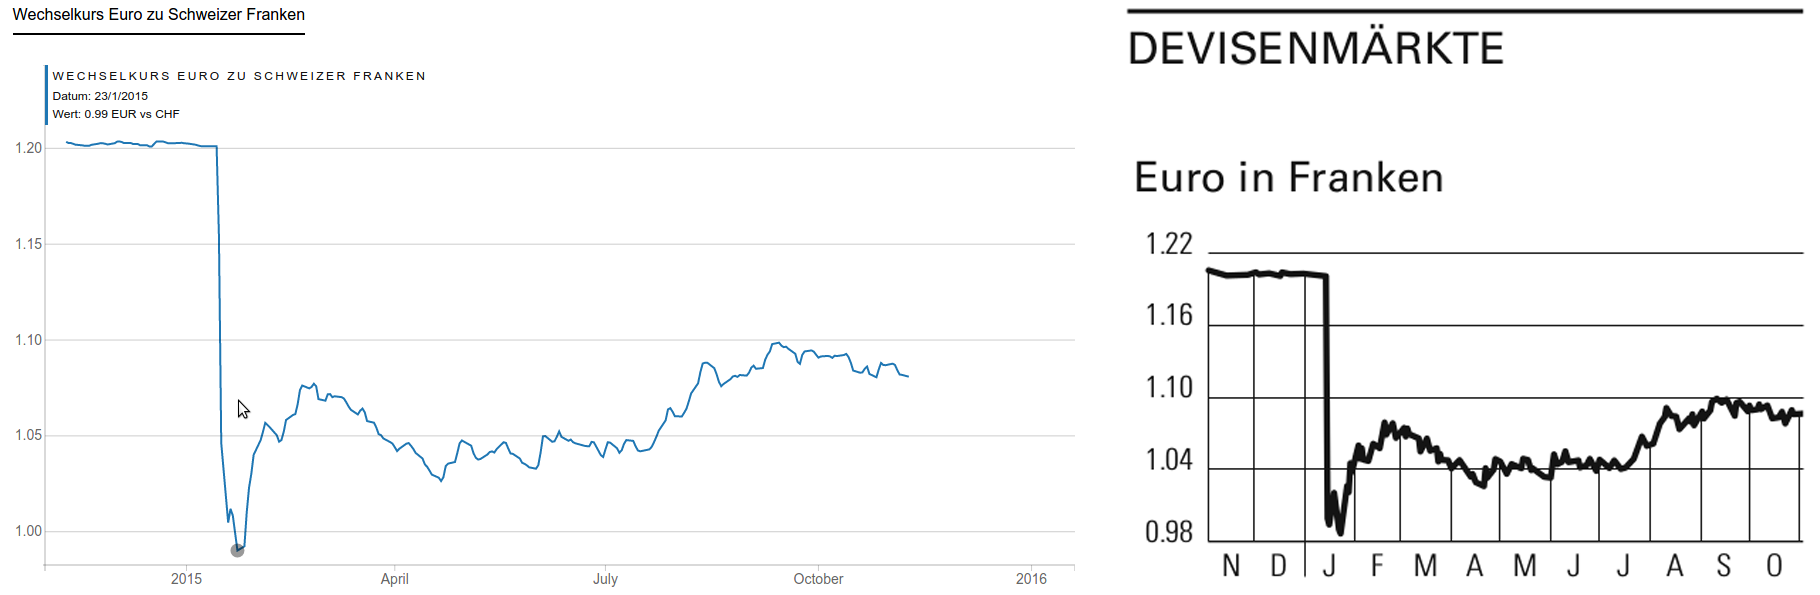
\includegraphics[width=\linewidth]{images/finance}
	\caption[Vergleich des dynamischen und statischen Diagramms]{Vergleich des dynamischen (links) und statischen Diagramms (rechts, NZZ 8.11.15) bei der Darstellung eines äquivalenten Datensatzes.}
	\label{fig:finance}
\end{figure}

Der Datensatz wird in beiden Beispielen in Abbildung \ref{fig:finance} mittels eines zweidimensionalen Liniendiagramm dargestellt. Man kann erkennen, dass es sich um denselben Datensatz handelt.

\subsection{Interaktion}

\paragraph{Verschiebung und Zoom.}

Beim dynamischen Diagramm ist es möglich durch Verschieben und Zoomen beliebige Bereiche des Diagramms vergrössert anzuzeigen. Somit kann der Benutzer zum Beispiel den Verlauf des Wechselkurses in einem Zeitraum von drei Tagen einsehen.

Im dynamischen Diagramm ist es so möglich, den genauen Verlauf des Wechselkurses während des Währungscrashs am 15. Januar und der folgenden Tagen zu analysieren; ein solches Vorgehen wäre beim statischen Diagramm nicht möglich.

\paragraph{Tooltip und Details auf Abruf.} 

Der Wert des Wechselkurses an einem bestimmten Tag kann abgerufen werden, indem der Benutzer mit der Maus in die Nähe eines bestimmten Datenpunktes fährt. In Bezug auf diesen Datensatz kann zum Beispiel das Datum ermittelt werden, an dem der Wechselkurs am tiefsten war.

Beim statischen Diagramm können keine genauen Werte abgelesen, sondern nur mit Hilfe der Achsenbeschriftungen abgeschätzt werden.

\subsection{Dynamik}

Da bei jedem Aufruf des dynamischen Diagramms der Datensatz neu geladen wird und anschliessend dargestellt wird, ist es möglich, den Datensatz stets zu aktualisieren. In dieser Applikation würde das zum Beispiel bedeuten, dass jeden Tag der neuste Datensatz der Börse verwendet werden und somit immer der aktuellste Kurs im Diagramm dargestellt werden würde.

Dies wurde nicht in dieser Applikation umgesetzt, jedoch wird dieses Prinzip zum Beispiel bei der interaktiven Kursanzeige von Yahoo \cite{yahoo} verwendet: Der Kurs wird jede Minute automatisch aktualisiert und angezeigt.

Da dynamische Diagramme im erweiterten Sinne Webapplikationen sind, die in einem Browser ausgeführt werden, können diese auch im Nachhinein mit einer praktisch unendlichen Anzahl Funktionen erweitert werden, da bei jedem Aufruf der Seite der Quellcode vom Server heruntergeladen wird.